\chapter{Results \& Discussions}
he present work focused on the preparation and functionalization of coconut fiber for fluoride adsorption studies. GTMAC-modified coconut fiber was prepared and adsorption experiments were planned using Design of Experiments (DOE) through Central Composite Design (CCD). Preliminary Langmuir adsorption model diagnostics were also carried out during Phase 2 of the study. This chapter presents the results obtained during biomaterial preparation, GTMAC functionalization, CCD experimental design, and Langmuir adsorption model analysis.  
\section{Biomaterial Preparation and GTMAC Functionalization}
Aaw coconut fiber was collected from a coir factory and used as the base adsorbent material for fluoride adsorption studies. The material was oven-dried at 80 °C for 2 hours to remove moisture content, followed by grinding using a mechanical grinder. The powdered material was sieved using 125 BSS mesh to obtain uniform particle size suitable for adsorption studies. Due to formation of fine powder during grinding and sieving, lower yield was obtained, and a total of 112 g of processed material was collected after preparation. 

Surface functionalization was carried out using Glycidyl Trimethyl Ammonium Chloride (GTMAC). Initially, the biomass was treated with NaOH solution overnight to remove lignin, hemicellulose, and surface impurities while activating cellulose hydroxyl groups for functionalization. Based on literature studies, 0.454 g of GTMAC per gram of biomass was used in approximately 50 mL solution. The reaction was carried out under alkaline conditions at pH 11–13 and maintained at 60 °C for 5 hours with sonication. The modified material was then washed to neutral pH and dried at 60 °C. 

\begin{figure}[H]
	\centering
	\begin{minipage}{0.45\textwidth}
		\centering
		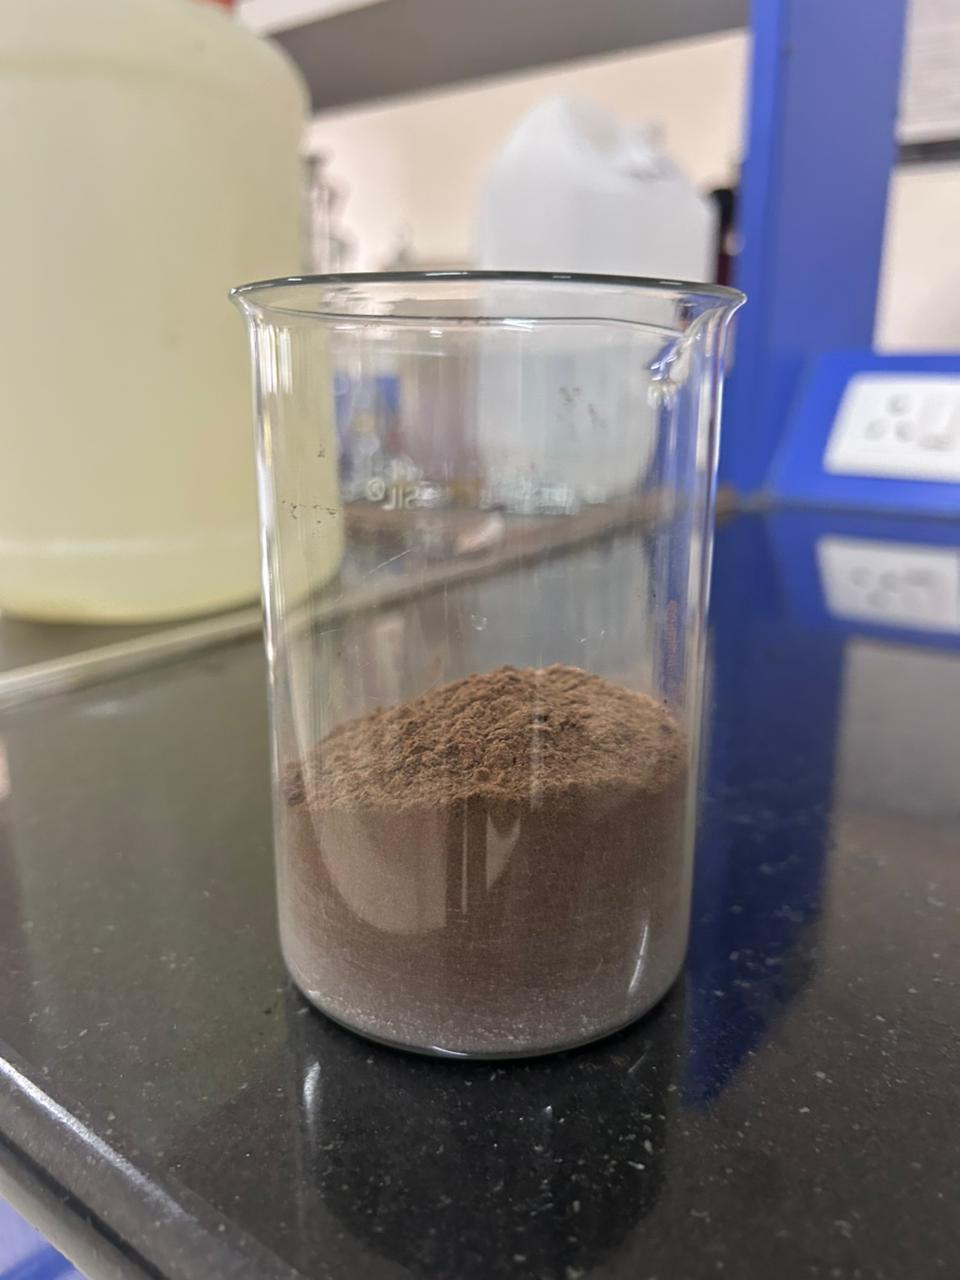
\includegraphics[width=\textwidth]{Chapter5/Figures/2.jpeg}
		\caption{Prepared bio material}
		\label{fig:bio1}
	\end{minipage}
	\hfill
	\begin{minipage}{0.45\textwidth}
		\centering
		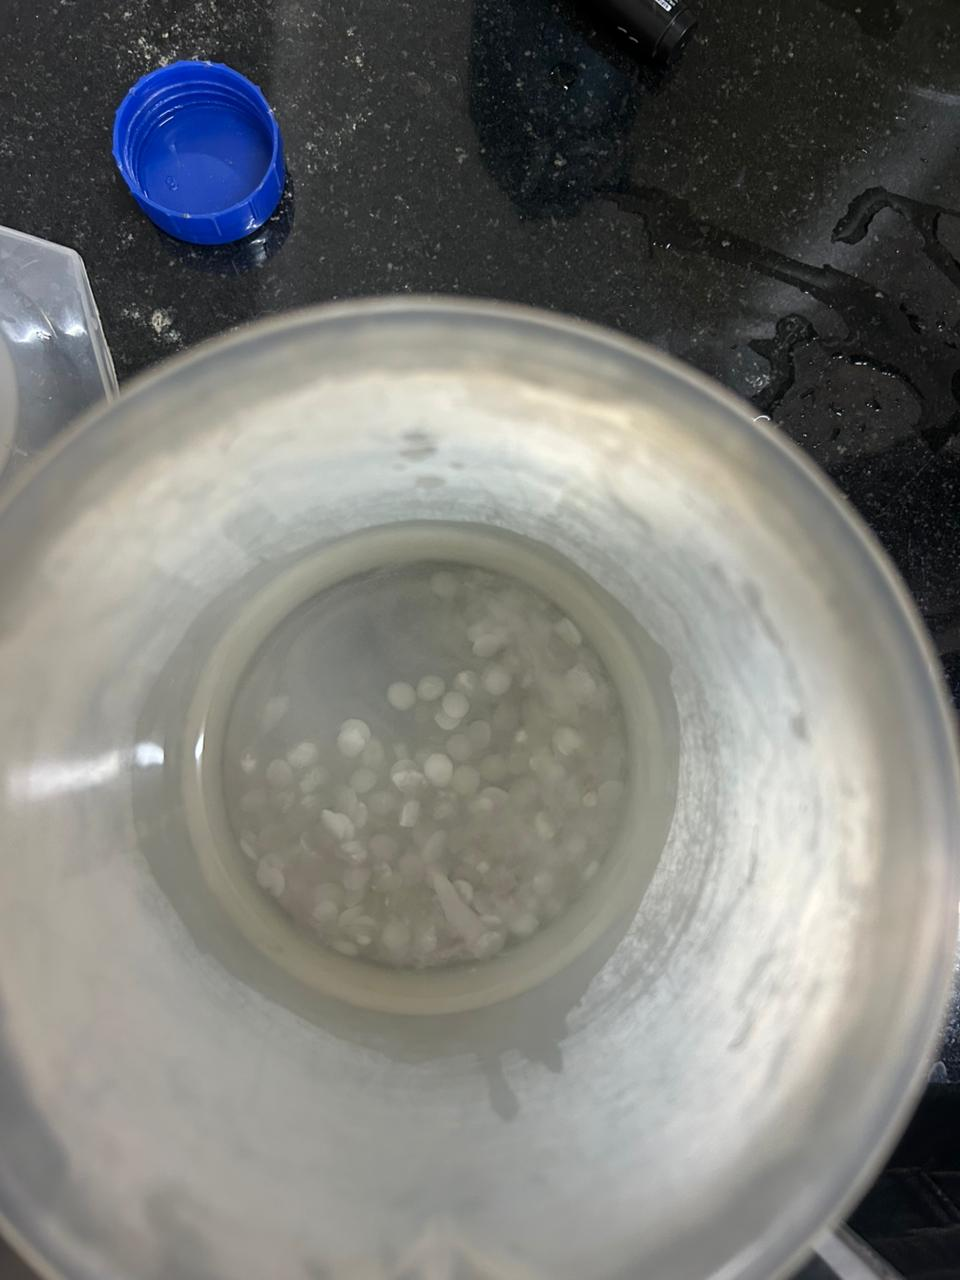
\includegraphics[width=\textwidth]{Chapter5/Figures/3.jpeg} 
		\caption{Preparation of 10\% NaOH solution}
		\label{fig:bio2}
	\end{minipage}
	
	\vspace{0.5cm}
	
	\begin{minipage}{0.45\textwidth}
		\centering
		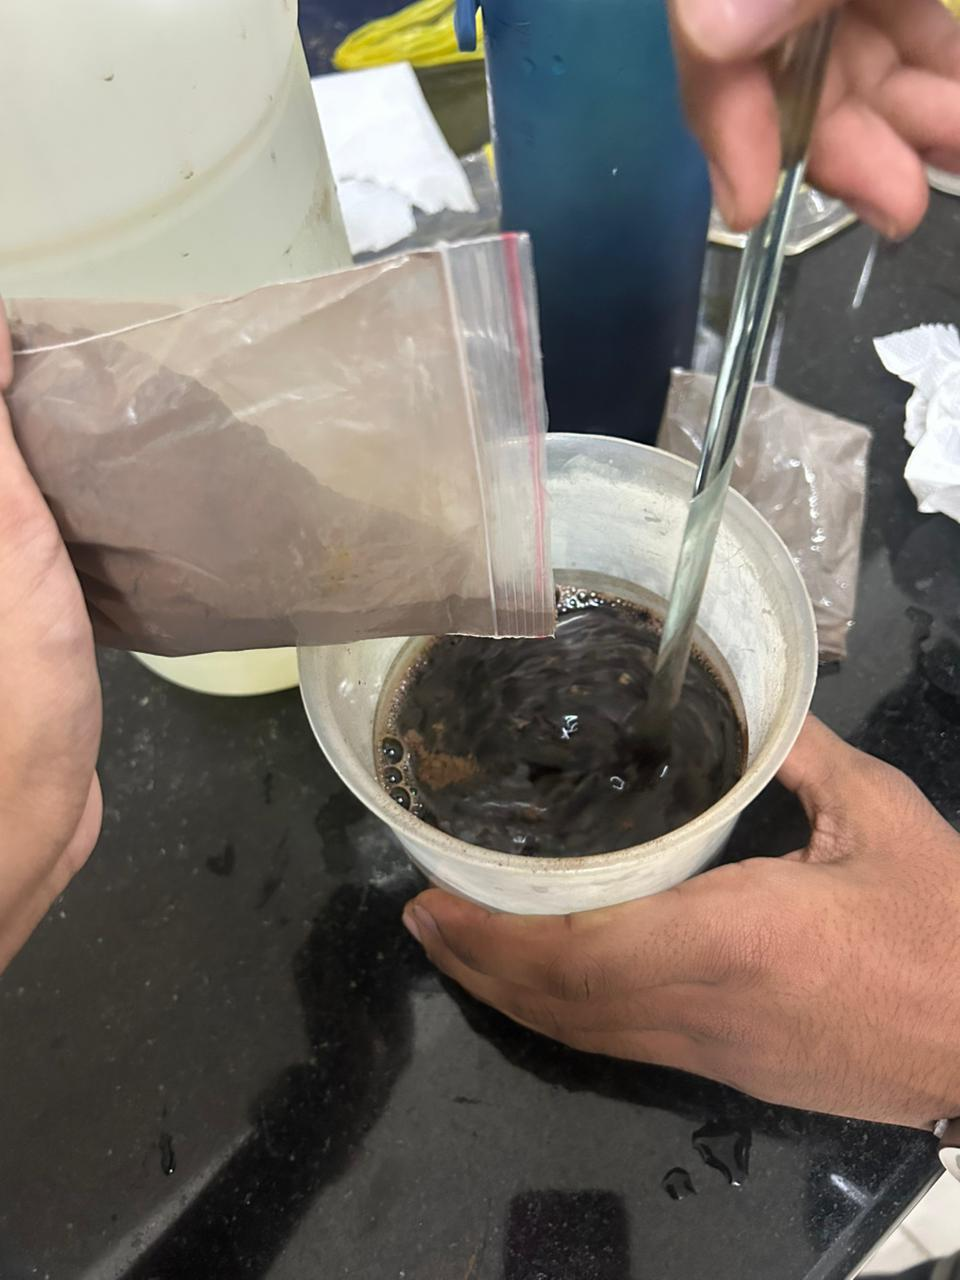
\includegraphics[width=\textwidth]{Chapter5/Figures/4.jpeg}
		\caption{Addition of biomass to 10 \%(w/v) NaOH solution}
		\label{fig:bio3}
	\end{minipage}
	\hfill
	\begin{minipage}{0.45\textwidth}
		\centering
		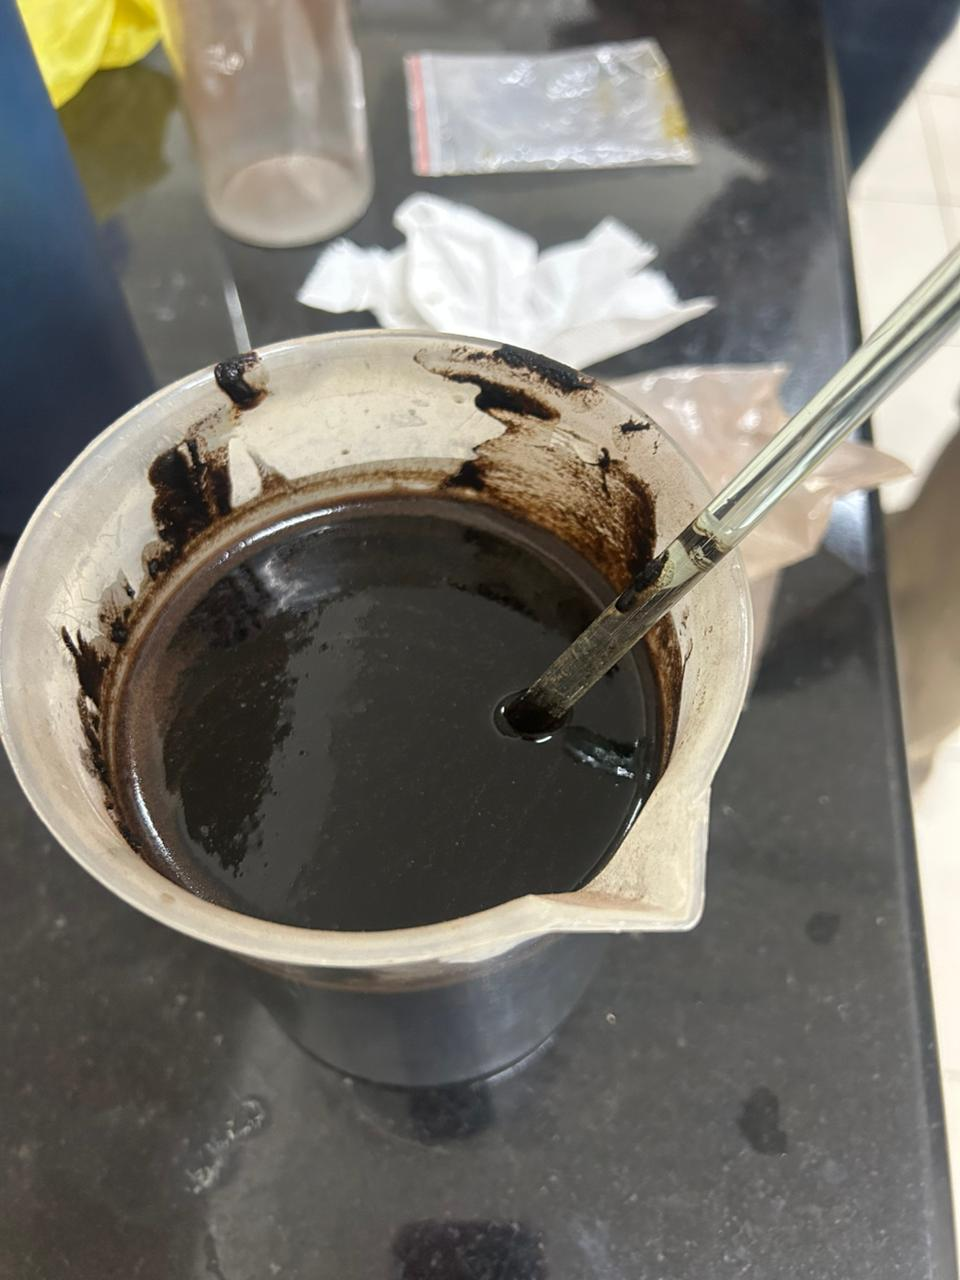
\includegraphics[width=\textwidth]{Chapter5/Figures/5.jpeg}
		\caption{Biomass in 10\% (w/v)NaOH solution}
		\label{fig:bio4}
	\end{minipage}
\end{figure}
\begin{figure}[H]
	\centering
	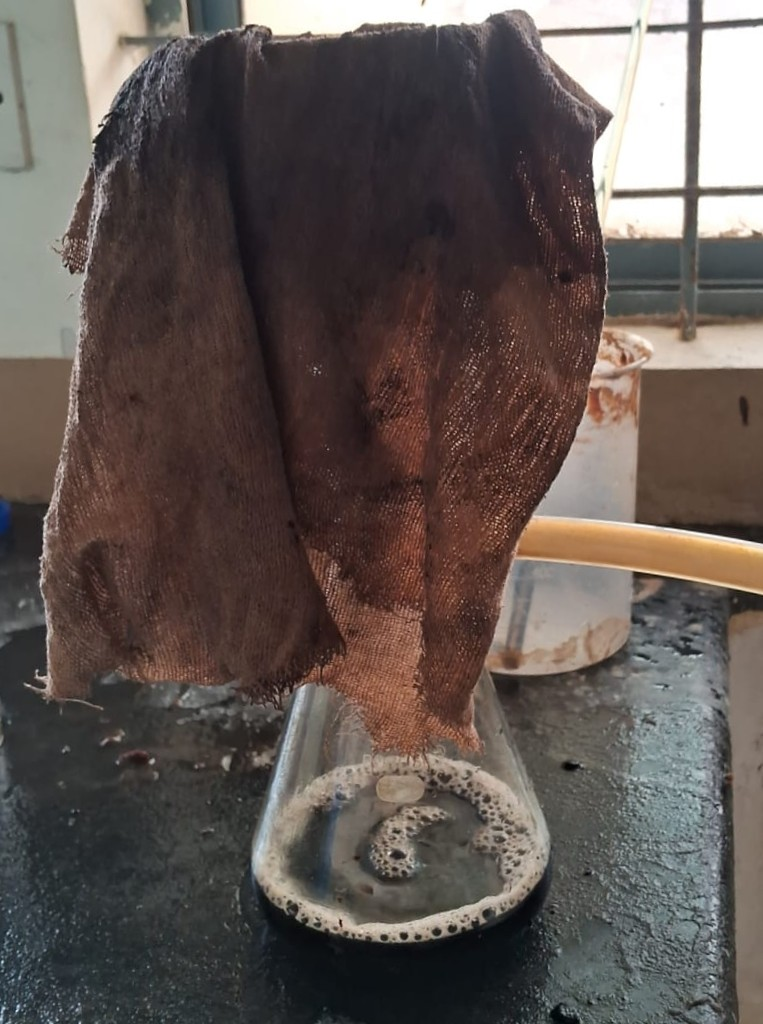
\includegraphics[width=0.5\textwidth]{Chapter5/Figures/9.jpeg}
	\caption{Washing of soaked biomass using distilled water}
	\label{fig:2.jpeg}
\end{figure}

\begin{figure}[H]
	\centering
	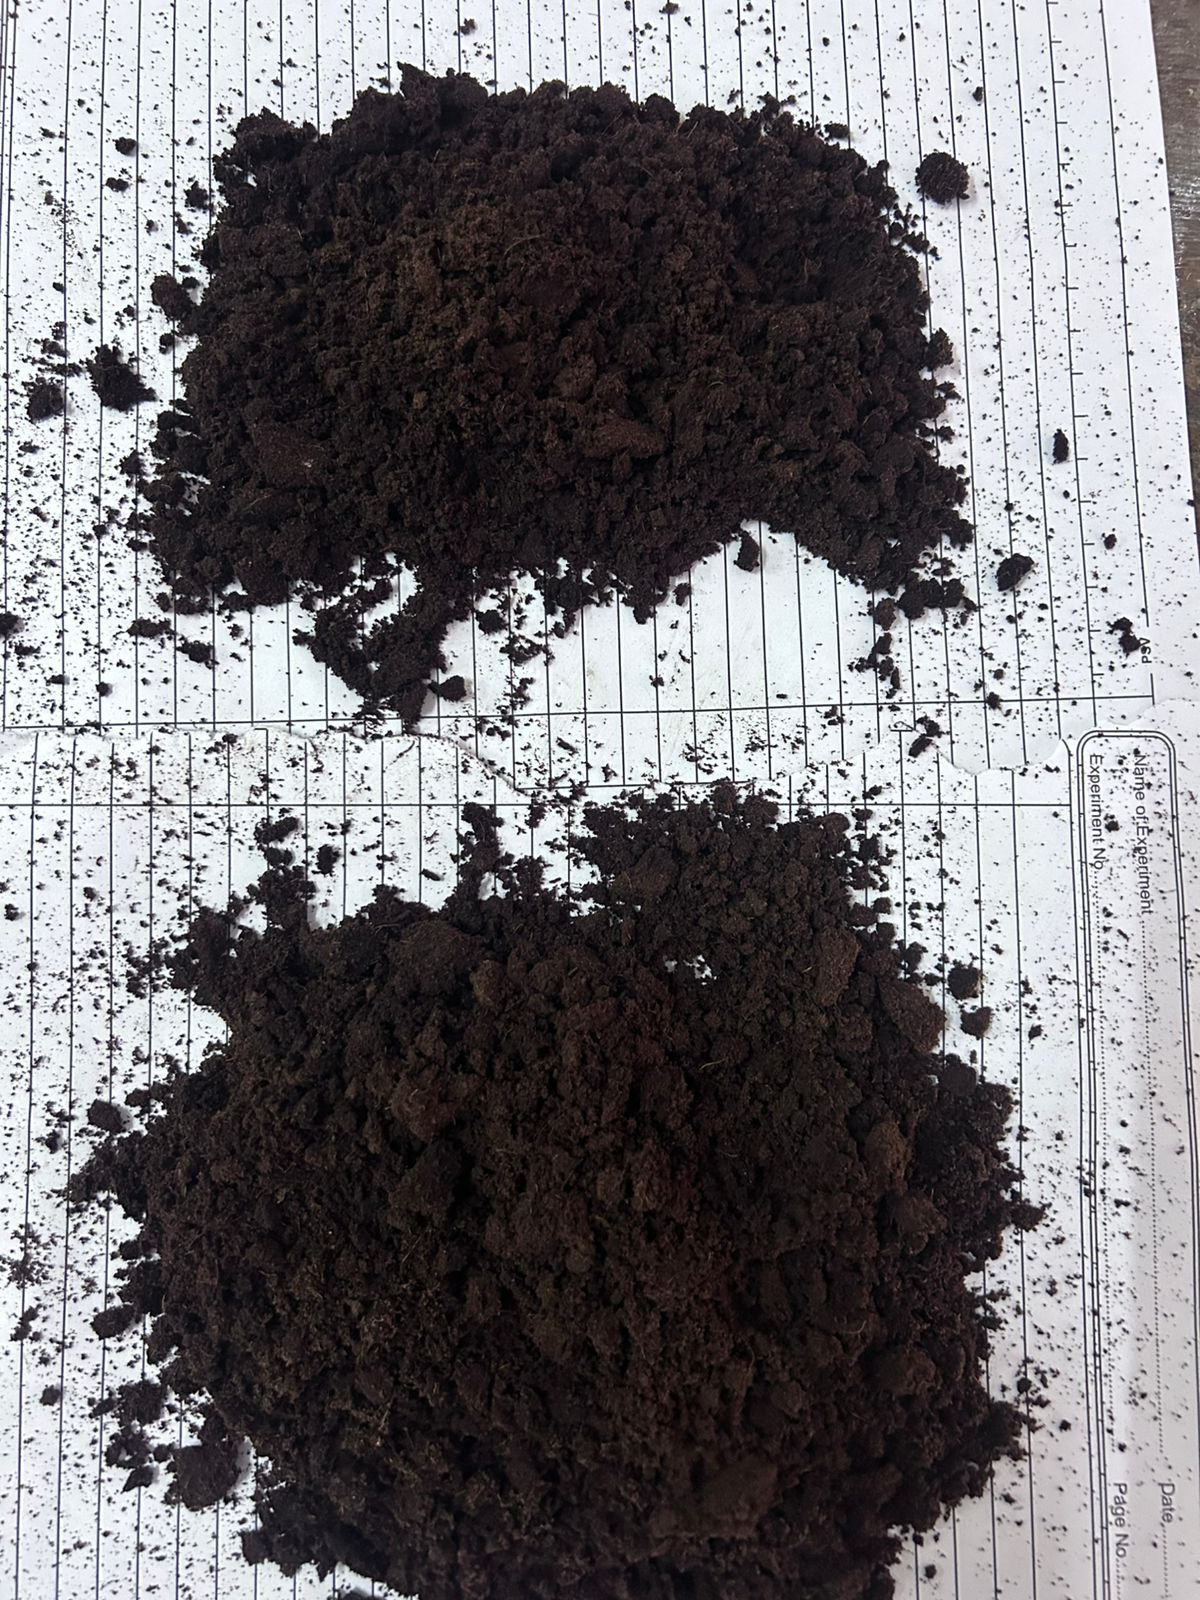
\includegraphics[width=0.5\textwidth]{Chapter5/Figures/10.jpeg}
	\caption{GTMAC modified material kept for drying}
	\label{fig:4.jpeg}
\end{figure}
%\begin{enumerate}
%\item Simulation results
%\item Experimental results
%\item Performance Comparison
%\item Inferences drawn from the results obtained
%\end{enumerate}
%All the figures should be properly explained by bringing the scenarios of the design done in the project. A detailed discussion of results obtained should be done in this chapter.
%
%\section{Tables in thesis}
%\begin{itemize}
%	\item All Table Caption should be in Sentence Case, TNR 10 Pt. It should be of the Format:
%	\begin{itemize}
%		\item Table 1.1 Results of the experiment ….(Centered)
%	\end{itemize}
%	\item It should be cited as Table 1.1.
%	\item Caption should appear above the Table.
%	\item Table Header and the entries should be of Font TNR 10 Pt, Justified.
%	\item For wider Table, the page orientation can be Landscape.
%	\item For Larger Table, it can run to pages and the header should be repeated for each page of the Table.
%	\item Table must be adjusted to fit in the page and no single row is left out for a new page.	
%\end{itemize}
%
%Sample Table \ref{c5:tab1} is given below for your reference,
%
%\begin{table}[htb]
%\fontsize{10}{12}\selectfont
%\caption{Country List}
%\label{c5:tab1}
%\begin{tabular}{|p{3cm}|c|c|c|}
%	%\hline
%	%\multicolumn{4}{|c|}{Country List} \\
%	\hline
%	\textbf{Country Name     or Area Name}& \textbf {ISO ALPHA 2 Code} & \textbf {ISO ALPHA 3 Code} & \textbf{ISO numeric Code}\\
%	\hline
%	\textbf{Afghanistan}   & AF    & AFG &   004\\\hline
%	\textbf{Aland Islands}&   AX  & ALA   & 248\\\hline
%	\textbf{Albania} & AL & ALB&  008\\\hline
%	\textbf{Algeria}    &DZ & DZA&  012\\\hline
%	\textbf{American Samoa}&   AS  & ASM&016\\\hline
%	\textbf{Andorra}& AD  & AND   & 020\\\hline
%	\textbf{Angola}& AO  & AGO& 024\\
%	\hline
%\end{tabular}
%\end{table}

%\begin{table}[htp]
%\fontsize{10}{12}\selectfont
%\centering
%\caption{Data units, sources, and dates} \label{c5:tab2}
%\begin{tabular}{| *4{>{\arraybackslash}m{1in}|} @{}m{0pt}@{}}
%	\hline
%	\textbf{Variable} & \textbf{Dates} & \textbf{Units} &
%	\textbf{Source}  &\\[2ex] 
%	\hline
%	\textbf{Nominal Physical Capital Stock} & 1950-1990 & Billions
%			US\$ & Nehru and Dhareshwar (1993) &\\[0ex]
%	\hline
%	\textbf{Total Population} & 1950-1990 & Billions & Nehru and
%			Dhareshwar (1993) &\\[0ex]
%	\hline
%	\textbf{Nominal GDP} & 1950-1990 & Billions  US\$ & PWT &\\[5ex]
%	\hline
%	\textbf{Real GDP per capita} & 1950-1990 & 2005 US\$ per capita & PWT &\\[5ex]
%	\hline
%\end{tabular}
%\end{table}

\section{Experimental Design and CCD Adsorption Runs}

The adsorption studies were planned using Design of Experiments (DOE) through 
Central Composite Design (CCD). Four major adsorption parameters were selected 
for the study:

\begin{itemize}
	\item pH
	\item Adsorbent dose
	\item Initial fluoride concentration
	\item Contact time
\end{itemize}
Approximately 30 CCD experimental runs were generated using Design-Expert software under different combinations of adsorption parameters. The generated CCD matrix provides systematic combinations of operating conditions for fluoride adsorption studies and optimization analysis. 
\begin{table}[H]
	\centering
	\caption{CCD experimental runs and fluoride removal response}
	\label{tab:ccd_results}
	\renewcommand{\arraystretch}{1.2}
	
	\resizebox{\textwidth}{!}{
		\begin{tabular}{cccccccc}
			\hline
			Std & Run & A:pH & 
			B:Adsorbent dose &
			C:Initial Fluoride & 
			D:Contact & Current & \% Fluoride \\
			&  & Factor 1 & g/100 mL &
			Concentration (ppm) &
			time (min) &
			percentage &
			removal \\
			\hline
			
			8  & 1  & 7   & 1    & 70 & 30  & 17.69 & 74.729 \\
			13 & 2  & 2   & 0.1  & 70 & 180 & 16.07 & 77.043 \\
			21 & 3  & 4.5 & 0.55 & 2  & 105 & 0.409 & 79.550 \\
			17 & 4  & 2   & 0.55 & 36 & 105 & 7.297 & 79.731 \\
			19 & 5  & 4.5 & 0.1  & 36 & 105 & 10.1  & 71.944 \\
			3  & 6  & 2   & 1    & 2  & 30  & 0.244 & 87.800 \\
			22 & 7  & 4.5 & 0.55 & 70 & 105 & 19.77 & 71.757 \\
			4  & 8  & 7   & 1    & 2  & 30  & 0.373 & 81.350 \\
			2  & 9  & 7   & 0.1  & 2  & 30  & 0.353 & 82.350 \\
			26 & 10 & 4.5 & 0.55 & 36 & 105 & 9.527 & 73.536 \\
			27 & 11 & 4.5 & 0.55 & 36 & 105 & 9.753 & 72.908 \\
			23 & 12 & 4.5 & 0.55 & 36 & 30  & 8.235 & 77.125 \\
			24 & 13 & 4.5 & 0.55 & 36 & 180 & 8.311 & 76.914 \\
			9  & 14 & 2   & 0.1  & 2  & 180 & 0.41  & 79.500 \\
			20 & 15 & 4.5 & 1    & 36 & 105 & 9.766 & 72.872 \\
			30 & 16 & 4.5 & 0.55 & 36 & 105 & 10.6  & 70.556 \\
			6  & 17 & 7   & 0.1  & 70 & 30  & 17.67 & 74.757 \\
			18 & 18 & 7   & 0.55 & 36 & 105 & 10.61 & 70.528 \\
			25 & 19 & 4.5 & 0.55 & 36 & 105 & 9.823 & 72.714 \\
			28 & 20 & 4.5 & 0.55 & 36 & 105 & 9.975 & 72.292 \\
			1  & 21 & 2   & 0.1  & 2  & 30  & 0.499 & 75.050 \\
			11 & 22 & 2   & 1    & 2  & 180 & 0.259 & 87.050 \\
			5  & 23 & 2   & 0.1  & 70 & 30  & 16.12 & 76.971 \\
			29 & 24 & 4.5 & 0.55 & 36 & 105 & 10.02 & 72.167 \\
			12 & 25 & 7   & 1    & 2  & 180 & 0.574 & 71.300 \\
			14 & 26 & 7   & 0.1  & 70 & 180 & 13.78 & 80.314 \\
			16 & 27 & 7   & 1    & 70 & 180 & 19.06 & 72.771 \\
			7  & 28 & 2   & 1    & 70 & 30  & 12.42 & 82.257 \\
			10 & 29 & 7   & 0.1  & 2  & 180 & 0.438 & 78.100 \\
			15 & 30 & 2   & 1    & 70 & 180 & 12.57 & 82.043 \\
			
			\hline
		\end{tabular}
	}
\end{table}
%All equation should be written using equation editor or using an equivalent tool.
%\begin{itemize}
%	\item Equations should be numbered as : 1.1, 1.2 ...
%	\item Equation should be Centered, 12 Pt, TNR. 
%	\item Equation number should be right Justified
%	\item It should be cited as Eqn. 1.1.
%   \item If the sentence starts by citing an equation, then it should be written as Equation 1.1 For example, Equation 5.1 states the Pythagoras theorem.
%
%	
%\end{itemize}
%
%For example in Eqn. \ref{eqn:pythag thm}, The well known Pythagorean theorem $x^2 + y^2 = z^2$ was 
%proved to be invalid for other exponents. 
%Meaning the next equation has no integer solutions:
%
%\begin{equation}
%\label{eqn:pythag thm}
%	x^n + y^n = z^n
%\end{equation}
%
%The mass-energy equivalence is described by the famous equation in Eqn. \ref{eqn:mass-eng}
%\begin{equation}
%\label{eqn:mass-eng}
%	E=mc^2
%\end{equation}
%
%discovered in 1905 by Albert Einstein. 

\section{Langmuir Adsorption Model Diagnostics}

%\vspace{2.5cm}
%
% \textbf{The chapters should not end with figures, instead bring the paragraph explaining about the figure at the end followed by a summary paragraph.}

Langmuir adsorption model diagnostics were carried out during Phase 2 of the study to evaluate adsorption prediction performance. The Langmuir adsorption equation is expressed as: 
\begin{equation}
	q_e = \frac{q_{\max} b C_e}{1 + b C_e}
\end{equation}

where:

\begin{itemize}
	\item $q_e$ = Equilibrium adsorption capacity (mg/g)
	\item $q_{\max}$ = Maximum monolayer adsorption capacity (mg/g)
	\item $b$ = Langmuir adsorption constant related to adsorption energy
	\item $C_e$ = Equilibrium fluoride concentration in solution (mg/L)
\end{itemize}

The diagnostic analysis included:

\begin{itemize}
	\item Actual vs Predicted plot
	\item Residual plot
	\item Residual distribution histogram
	\item Q-Q probability plot
\end{itemize}
\begin{figure}[H]
	\centering
	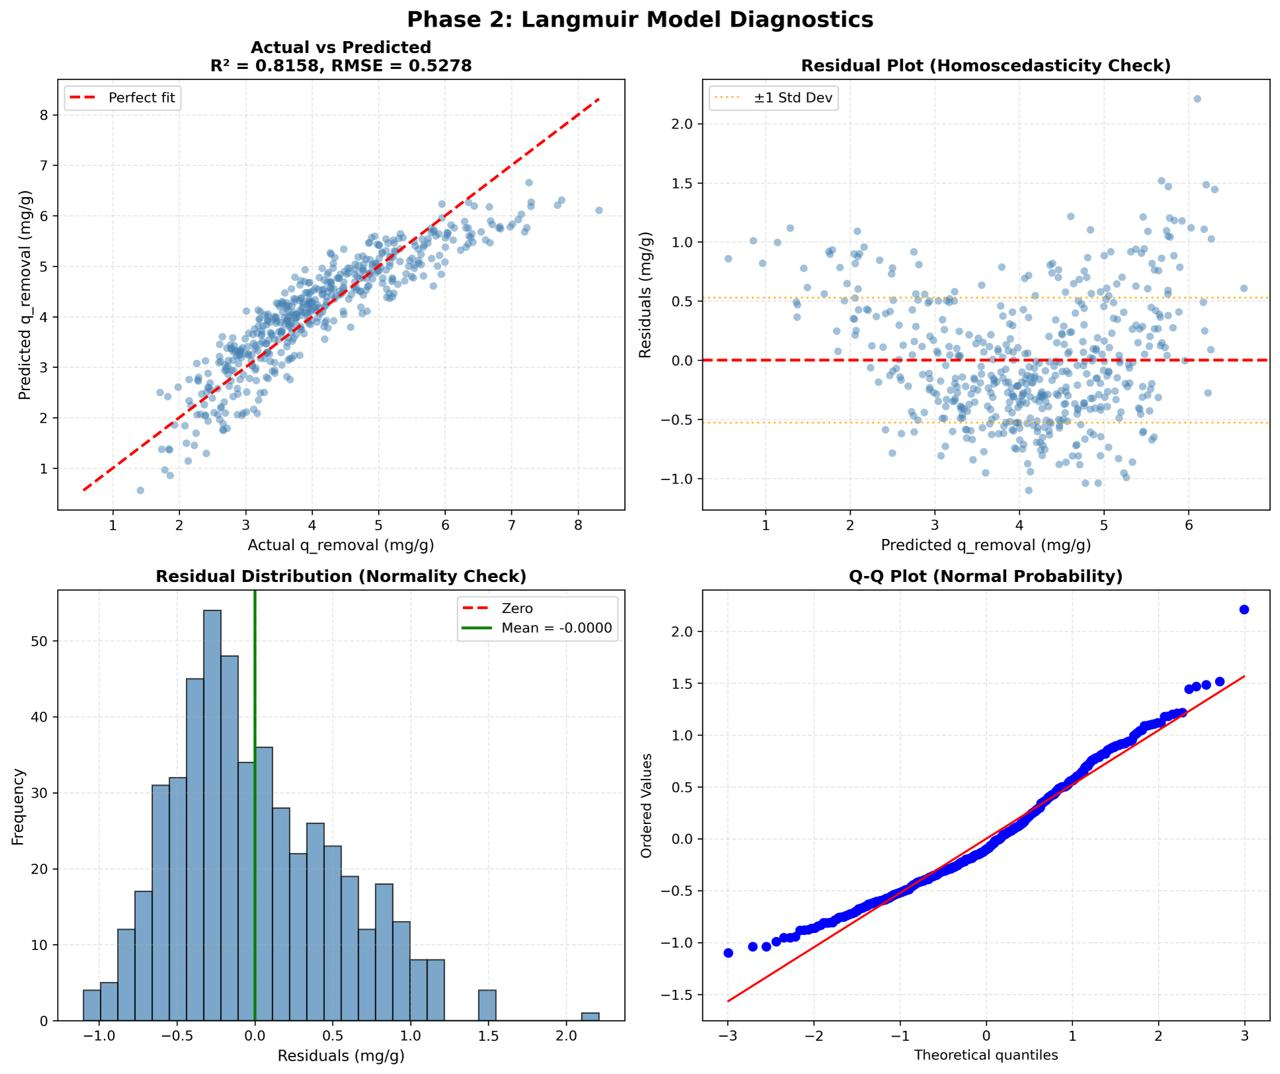
\includegraphics[width=0.7\textwidth]{Chapter5/Figures/6.jpeg}
	\caption{Graphs from the model built}
	\label{fig:label}
\end{figure}


